
The three different algorithms discussed in section XXX was implemented in
\href{https://github.com/erikfsk/fysstk4155-project-1/blob/master/project/project-e.py}{\color{blue}{our script}}.
It is a few different versions, but the \"e\" version contains all you need.
All the scripts discussed in this report can be found at
\href{https://github.com/erikfsk/fysstk4155-project-1/}{\color{blue}{our github}}.
\\
\\
This part of the report is meant as a part where we show that our program works as
we expected. We will look at how our implementation compare to Scikit's, how time increase as we increase
the order we fit and how the modul crumbles as we add noise to our data.
\\
\\
The program was tested on the Frank-function, see equation \ref{eq:Franke}.
With an known solution we did a k-fold test and an degree and $\lambda$/$\alpha$ test.
Both tested was done with the script descriped earlier.
The tables below shows the different results.

\begin{align}
f(x,y) &=
\frac{3}{4} e^{\left(-\frac{(9x-2)^2}{4} - \frac{(9y-2)^2}{4}\right)}
+\frac{3}{4} e^{\left(-\frac{(9x+1)^2}{49}- \frac{(9y+1)}{10}\right)}
+\frac{1}{2} e^{\left(-\frac{(9x-7)^2}{4} - \frac{(9y-3)^2}{4}\right)}
 -\frac{1}{5} e^{\left(-(9x-4)^2 - (9y-7)^2\right)}
\label{eq:Franke}
\end{align}

\subsection{Scikit vs. manually implementation}

Our implementation was verified with Scikit's OLS solution. The figur below shows
the result from the comparison.

\begin{figure}[H]
    \centering
    \begin{subfigure}{0.5\textwidth}
        \centering
        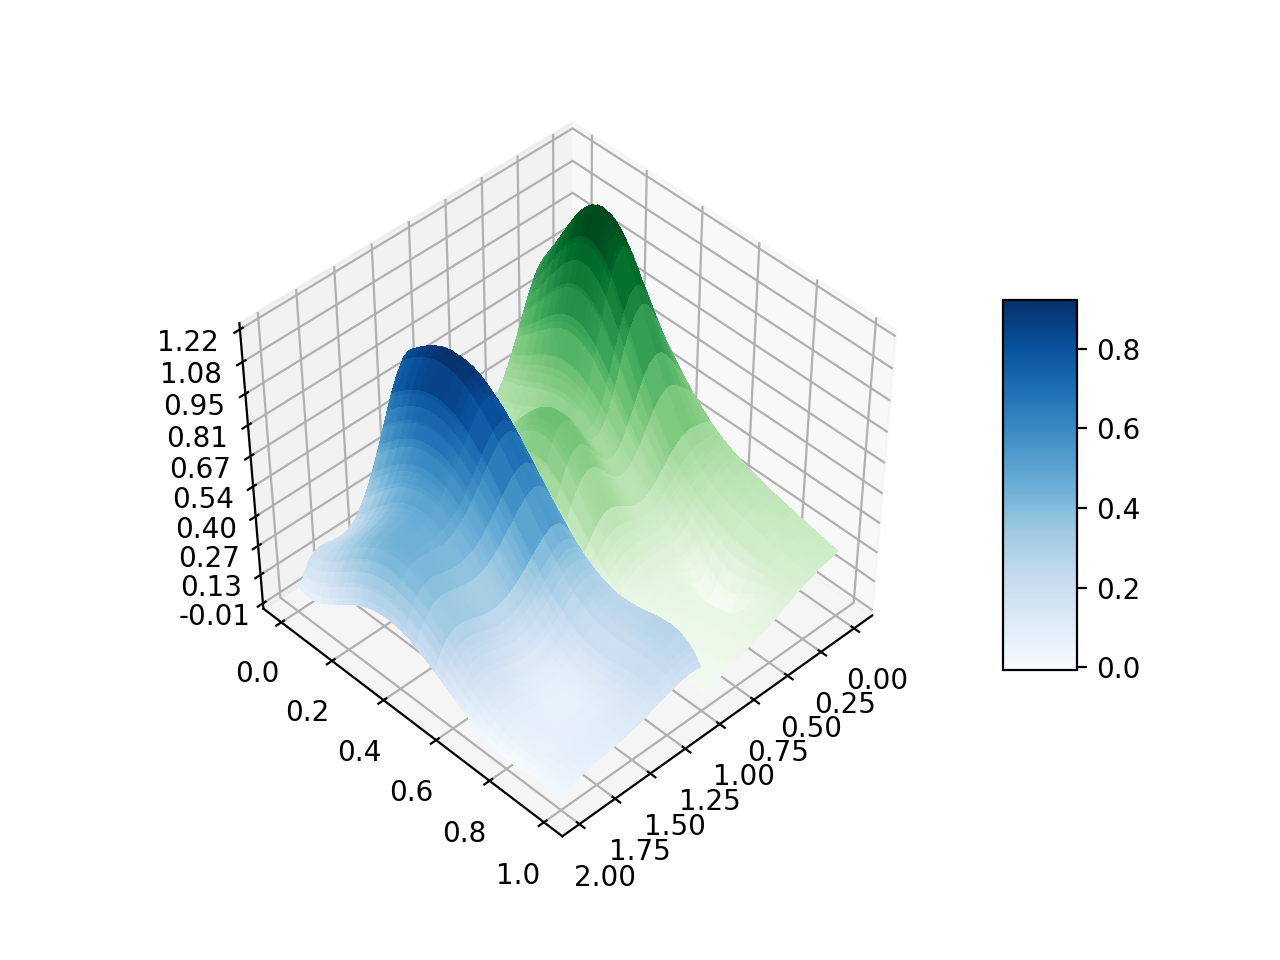
\includegraphics[width=\linewidth]{method/bilder/actual}
        \caption{}
    \end{subfigure}%
    ~
    \begin{subfigure}{0.5\textwidth}
        \centering
        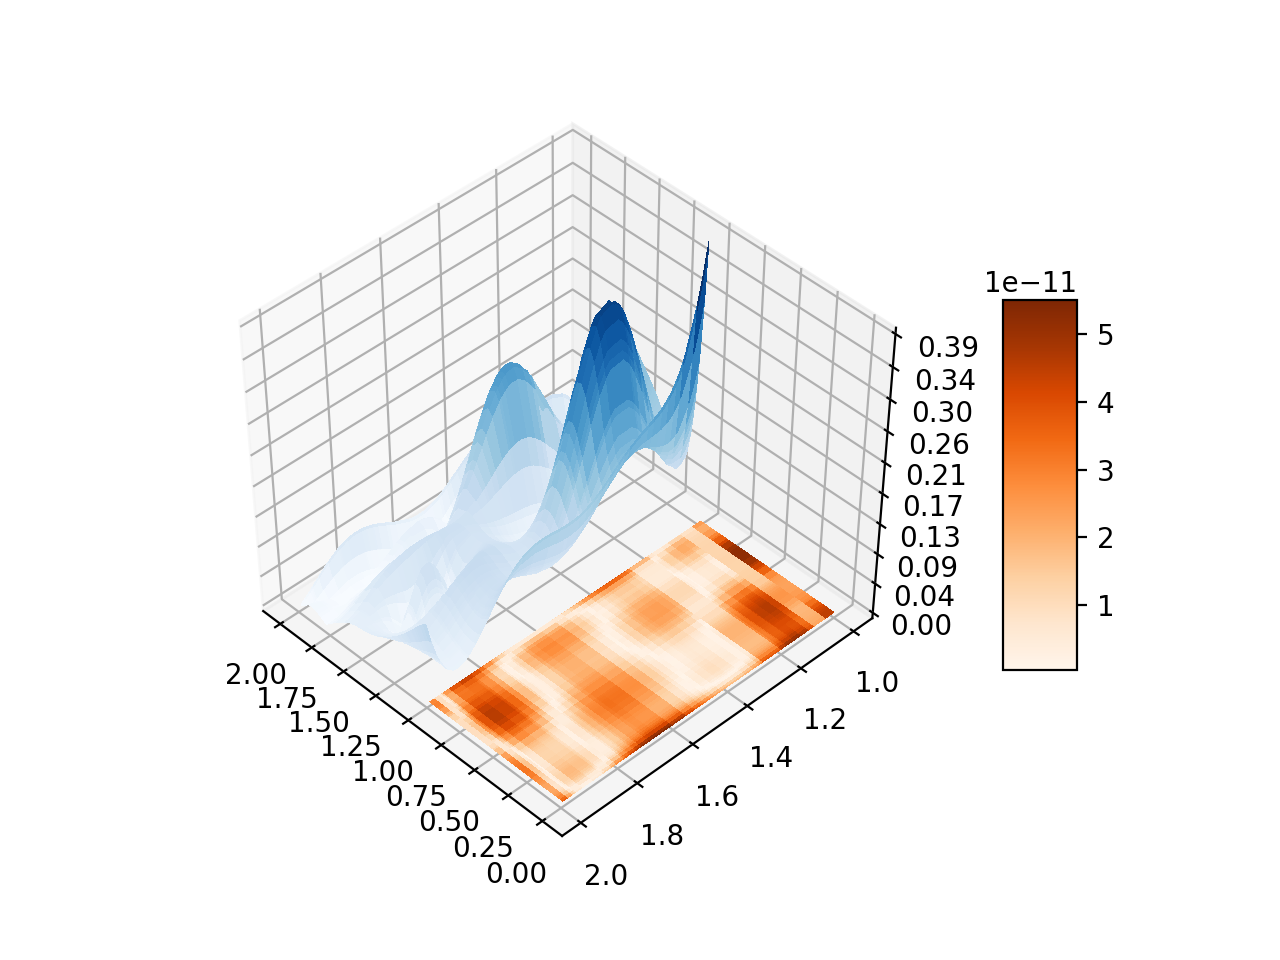
\includegraphics[width=\linewidth]{method/bilder/error}
        \caption{}
    \end{subfigure}
    \caption{a)Shows the \color{green} Franke function\color{black}, equation \ref{eq:Franke}, as it is.
    The \color{blue}OLS implementation \color{black} was used on the Franke function with noise.
    The result is shown as the blue graph.
    b)The \color{blue}blue \color{black} graph is the error compared to the actual Franke function,
    not the dataed that OLS were trained on. The \color{orange} orange \color{black} graph is the absolute error
    for our OLS compared to Scikit's.}
    \label{fig:test}
\end{figure}

\pagebreak
\subsection{Time evolution}



\begin{center}
\label{tab:time-test}
\captionof{table}{This tables shows how time develops as a function of order fitted.
One should not be suprised that Scikit has a faster algorithm, than us.
The $_{relative}$ means that it is as fraction of the second order fit time.
For lasso and ridge the $\lambda$/$\alpha$ was set to 1e-5. It is expected for higher order fits
to have longer calculation time, because the matrix $\textbf{X}$ will get bigger. This is
exactly what we see with our program.}
\begin{tabularx}{\textwidth}{l X c X c X c X c X c}
    \hline
    \hline
        degree $\downarrow$ && method $\rightarrow$ && OLS && SCIKIT && RIDGE && SCIKIT LASSO\\
    \hline
        $2  $               && &&   0.01517s &&	0.25830s	 &&	0.00516s      && 0.00543s		\\
        $2_{relative}$   	&& &&   1.00   	 &&	1.00 	     &&	1.00          &&	1.00	\\
        $3_{relative}$   	&& &&   2.42   	 &&	1.58	     &&	2.45          &&	2.38	\\
        $4_{relative}$   	&& &&   3.63   	 &&	2.45	     &&	5.11          &&	4.88	\\
        $5_{relative}$   	&& &&   4.98   	 &&	3.61	     &&	8.77          &&	8.31	\\
    \hline
\end{tabularx}
\end{center}

\subsection{Noise - MSE \& R2 evolution}



\begin{center}
\label{tab:noise-test-MSE}
\captionof{table}{This tables shows how the MSE evoles for different amount of noise.
As described in section \ref{sec:normal}, the Z data is normalized, so the MSE is 0.00127, when the highest values are 1.
Which means that we have at least an error of 0.1\% for the implementation on Franke function
without noise. The $_{relative}$ means that it is as fraction of the zero noise data's MSE.
For lasso and ridge the $\lambda$/$\alpha$ was set to 1e-5 and it was a fifth order fitting for all
of the methods. The MSE grows as the noise increase to 50\% of the data, which is expected!}
\begin{tabularx}{\textwidth}{l X c X c X c X c X c}
    \hline
    \hline
        Noise level $\downarrow$ && method $\rightarrow$ && OLS && SCIKIT && RIDGE && SCIKIT LASSO\\
    \hline
        $0  $               && &&   0.00127     &&	0.00127	  &&	0.00514      && 0.00127		\\
        $0_{relative}$   	&& &&   1.00   	    &&	1.00 	  &&	1.00         &&	1.00	\\
        $0.01_{relative}$   && &&   1.03   	    &&	1.03	  &&	1.00         &&	1.03	\\
        $0.2_{relative}$   	&& &&   12.84   	&&	12.84	  &&	3.68         &&	12.84	\\
        $0.5_{relative}$   	&& &&   42.04   	&&	42.04	  &&	10.84        &&	42.04	\\
    \hline
\end{tabularx}
\end{center}

\begin{center}
\label{tab:noise-test-R2}
\captionof{table}{This tables shows how the R2 score evoles for different amount of noise.
For lasso and ridge the $\lambda$/$\alpha$ was set to 1e-5 and it was a fifth order fitting for all
of the methods. Ideally we would want an R2 score of 1 for zero noise.
The R2 score shrinks as the noise increase to 50\% of the data, which is expected!}
\begin{tabularx}{\textwidth}{l X c X c X c X c X c}
    \hline
    \hline
        Noise level $\downarrow$ && method $\rightarrow$ && OLS && SCIKIT && RIDGE && SCIKIT LASSO\\
    \hline
        $0$   	    && &&   0.98  	&&	0.98	  &&   0.91         &&	0.98    \\
        $0.01$      && &&   0.98  	&&	0.98      &&   0.91         &&	0.98    \\
        $0.2$   	&& &&   0.68   	&&	0.68	  &&   0.62         &&	0.68	\\
        $0.5$   	&& &&   0.28   	&&	0.28	  &&   0.25        &&	0.28	\\
    \hline
\end{tabularx}
\end{center}
